%!TEX root = ../talk.tex

\section{Comparison}\label{sec:numer}

%%%

\frameinlbffalse

{
\usebackgroundtemplate{
\tikz[overlay,remember picture] \node[opacity=0.4, at=(current page.center)] {
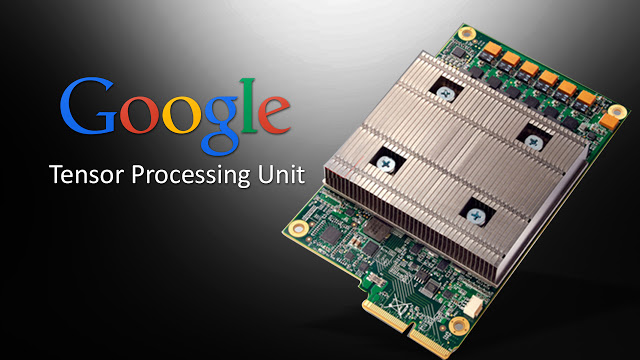
\includegraphics[width=1.15\paperwidth,height=0.675\paperwidth]{figures/tpu.jpg}
};}

\begin{frame}[plain]
\frametitle{\S\ref{sec:numer}. \insertsection}
\listofframes
\end{frame}
\addtocounter{framenumber}{-1} % this page does not count

}

\frameinlbftrue


%%%
\subsection{Test setting}
%%%

\begin{frame}
	\MyLogo
	\frametitle{Hardware Platforms}  

\smallskip 

\begin{itemize}

\item CPU: one quad-core desktop CPU (Intel i7-3820 CPU
		@3.60GHz) and two 8-core server-grade CPUs (Intel
		Xeon CPU E5-2630 v3 @2.40GHz)
		
\item GPU: GTX 1080 @1607MHz with
		Pascal architecture, and Telsa K80 @562MHz with Kepler
		architecture 
	\end{itemize}
	
\begin{figure}[htbp] 
	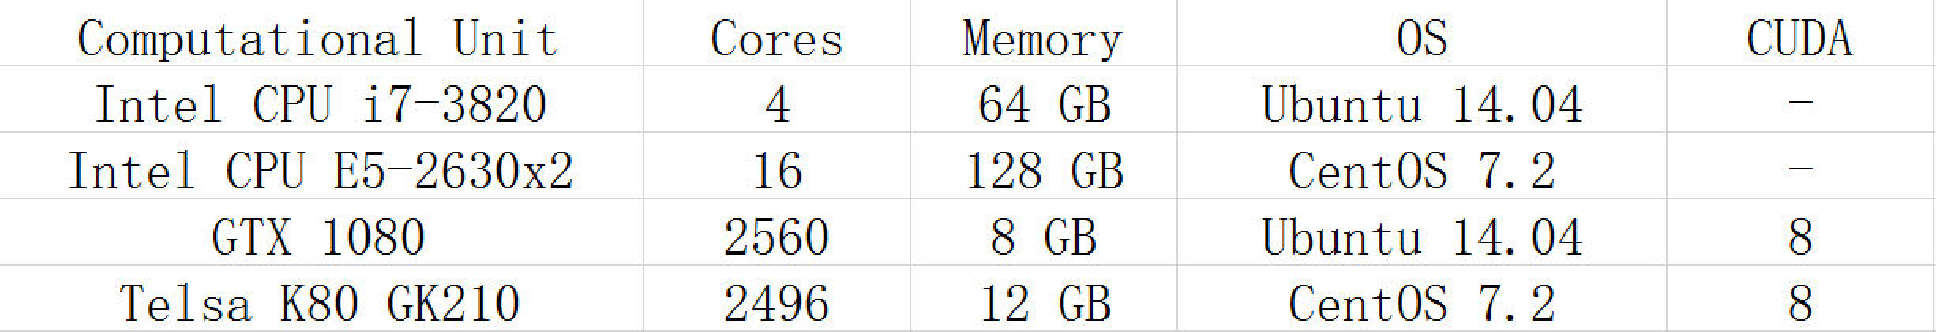
\includegraphics[height=1.3in]{figures/platforms.pdf} 
	\caption{The experimental hardware settings for numerical tests}
\end{figure}
	
\begin{center}
{\color{red} \scriptsize
Benchmarking State-of-the-Art Deep Learning Software Tools, by S.-H. Shi, et al., arXiv, 2017}
\end{center}

\end{frame}

%%%

\begin{frame}
  \MyLogo
  \frametitle{Neural Networks and Test Data Sets}  

\medskip

\begin{itemize}

\item A large fully-connected neural network (\alert{FCN-S}) with around 55 million parameters is used to evaluate the performance of FCN

\item The classical AlexNet (\alert{AlexNet-S}) is used as an representative of CNN

\item A smaller FCN (\alert{FCN-R}) is constructed for MNIST data set

\item An AlexNet (\alert{AlexNet-R}) architecture is used for Cifar10 data set

\item For RNNs, considering that the main computation complexity is related to the length of input sequence, 2 LSTM layers with input length of 32.

\end{itemize}

\begin{figure}[htbp] 
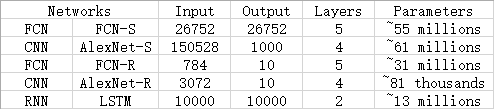
\includegraphics[height=1in]{figures/models.png} 
\caption{The experimental setup of neural networks for synthetic and real data}
\end{figure}
	
\end{frame}

%%%
\subsection{CPU tests}
%%%

\begin{frame}
	\MyLogo
	\frametitle{CPU Scalability: FCN Synthetic}  
	\begin{figure}[htbp] 
		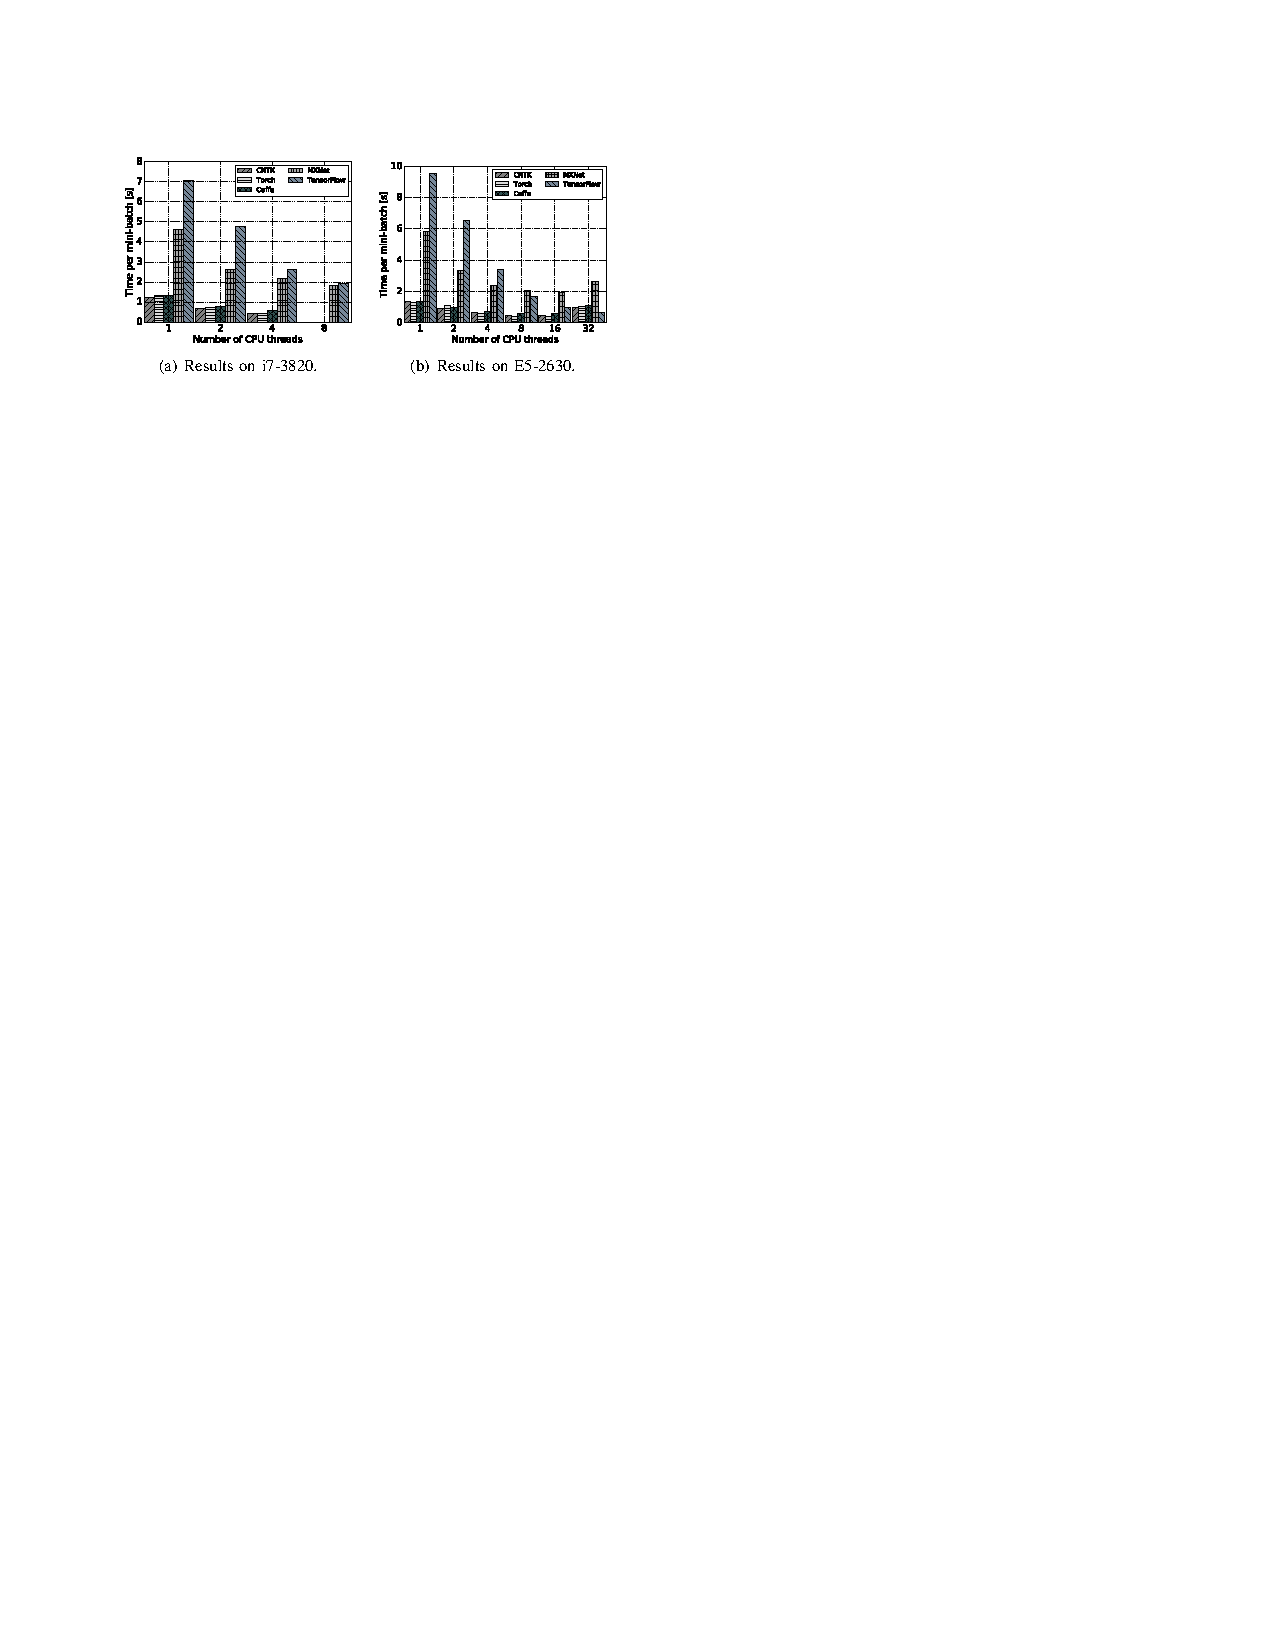
\includegraphics[width=\linewidth]{figures/FCN-S1.pdf} 
		\caption{FCN-S performance comparison on CPU platform with a mini-batch size of 64 (The lower the better)}
	\end{figure}
\end{frame}

%%%

\begin{frame}
	\MyLogo
	\frametitle{CPU Scalability: FCN Real}  
	\begin{figure}[htbp] 
		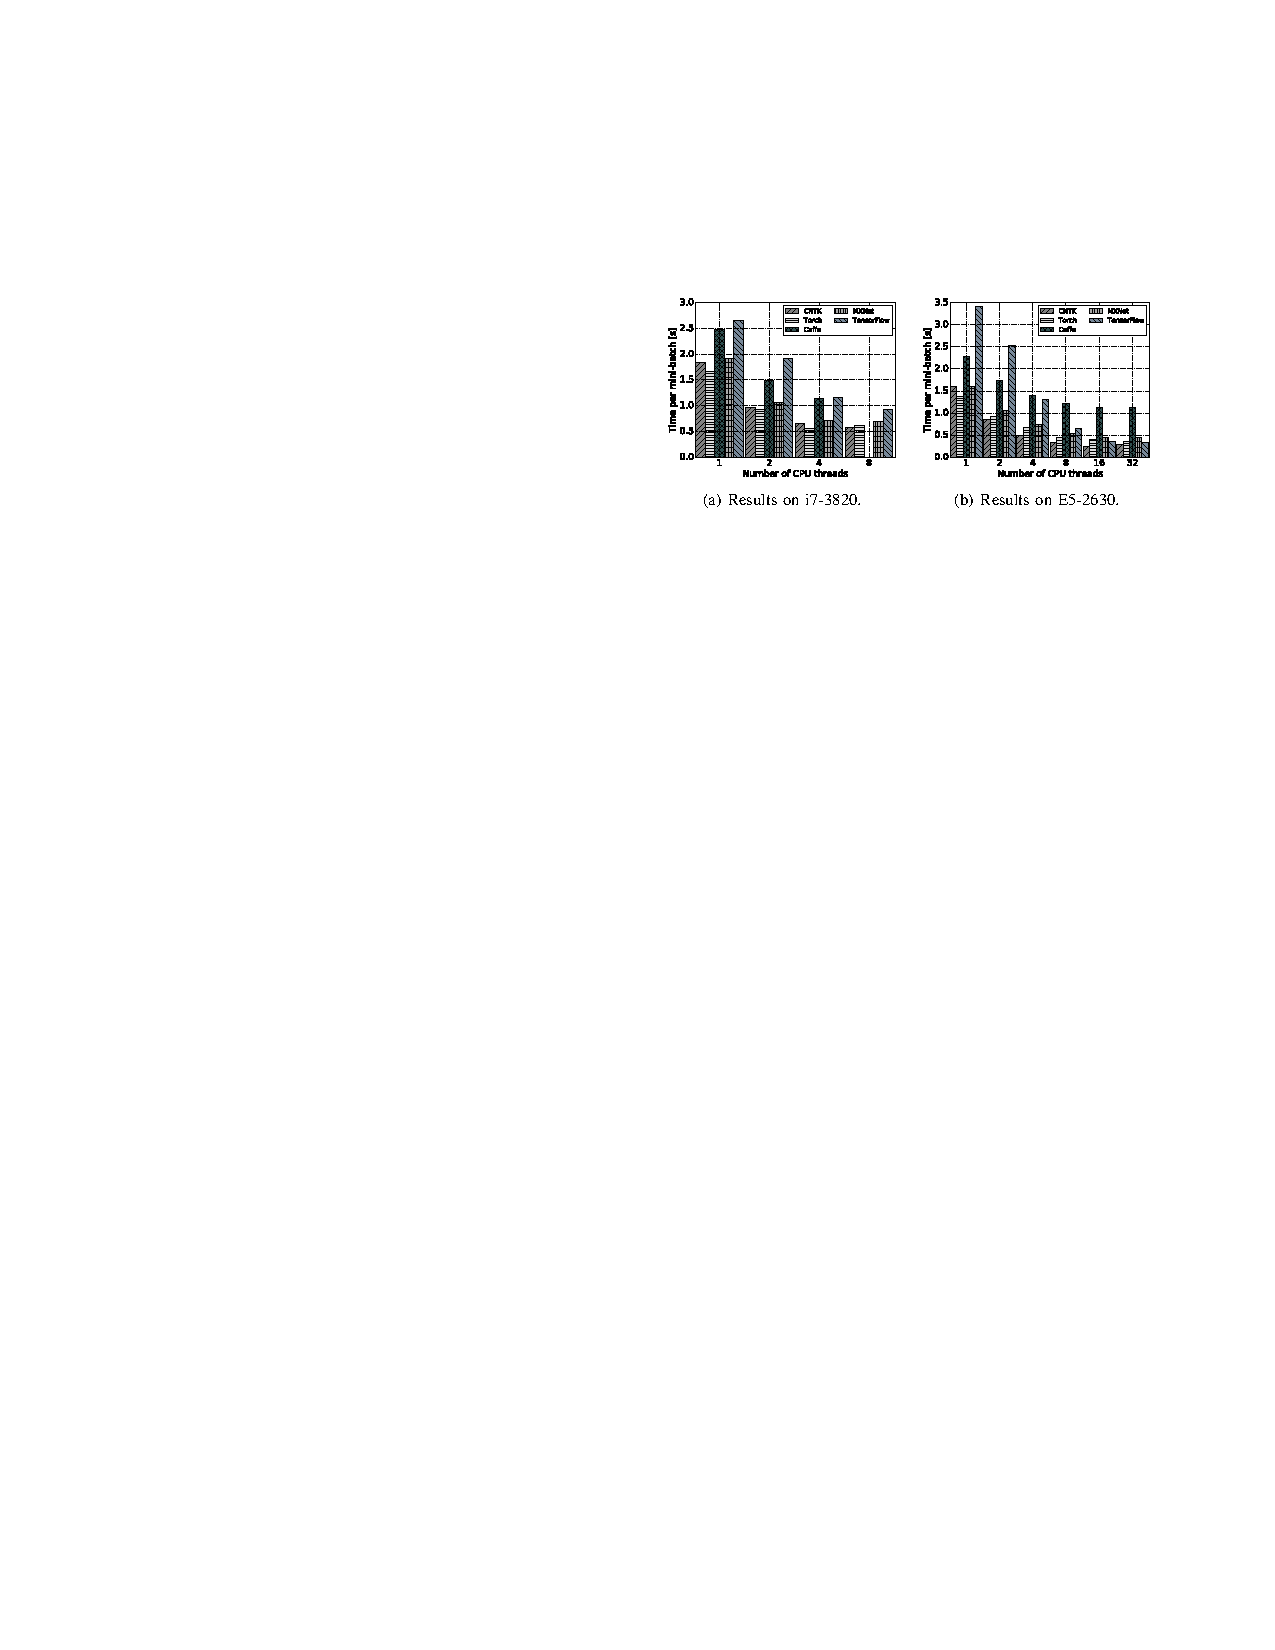
\includegraphics[width=\linewidth]{figures/FCN-R1.pdf} 
		\caption{The FCN-R performance comparison on CPU platform with a mini-batch size of 1024 (The lower the better)}
	\end{figure}
\end{frame}

%%%

\begin{frame}
	\MyLogo
	\frametitle{CPU Scalability: CNN Synthetic}  

	\begin{figure}[htbp] 
		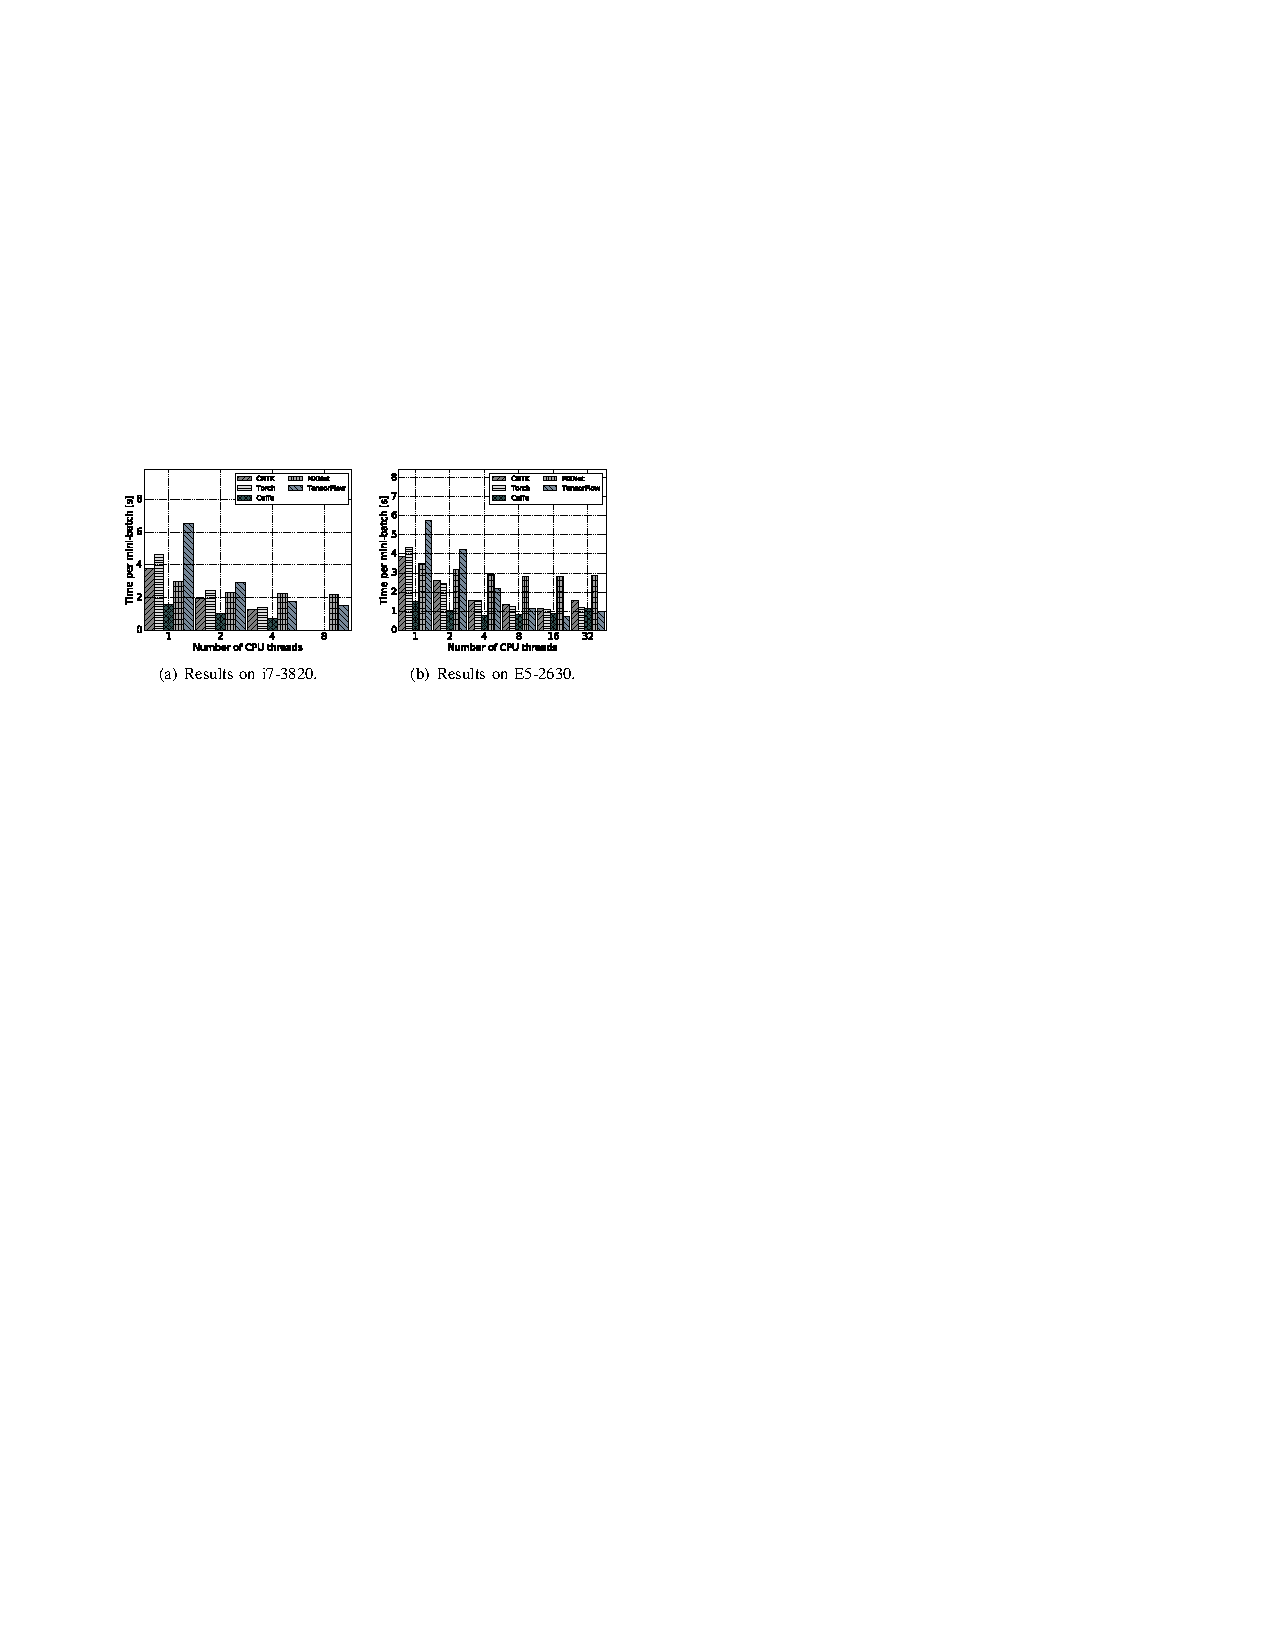
\includegraphics[width=\linewidth]{figures/AlexNet-S1.pdf} 
		\caption{AlexNet-S performance comparison on CPU platform with a mini-batch size of 16 (The lower the better)}
	\end{figure}	
\end{frame}

%%%

\begin{frame}
	\MyLogo
	\frametitle{CPU Scalability: CNN Real}  
	\begin{figure}[htbp] 
		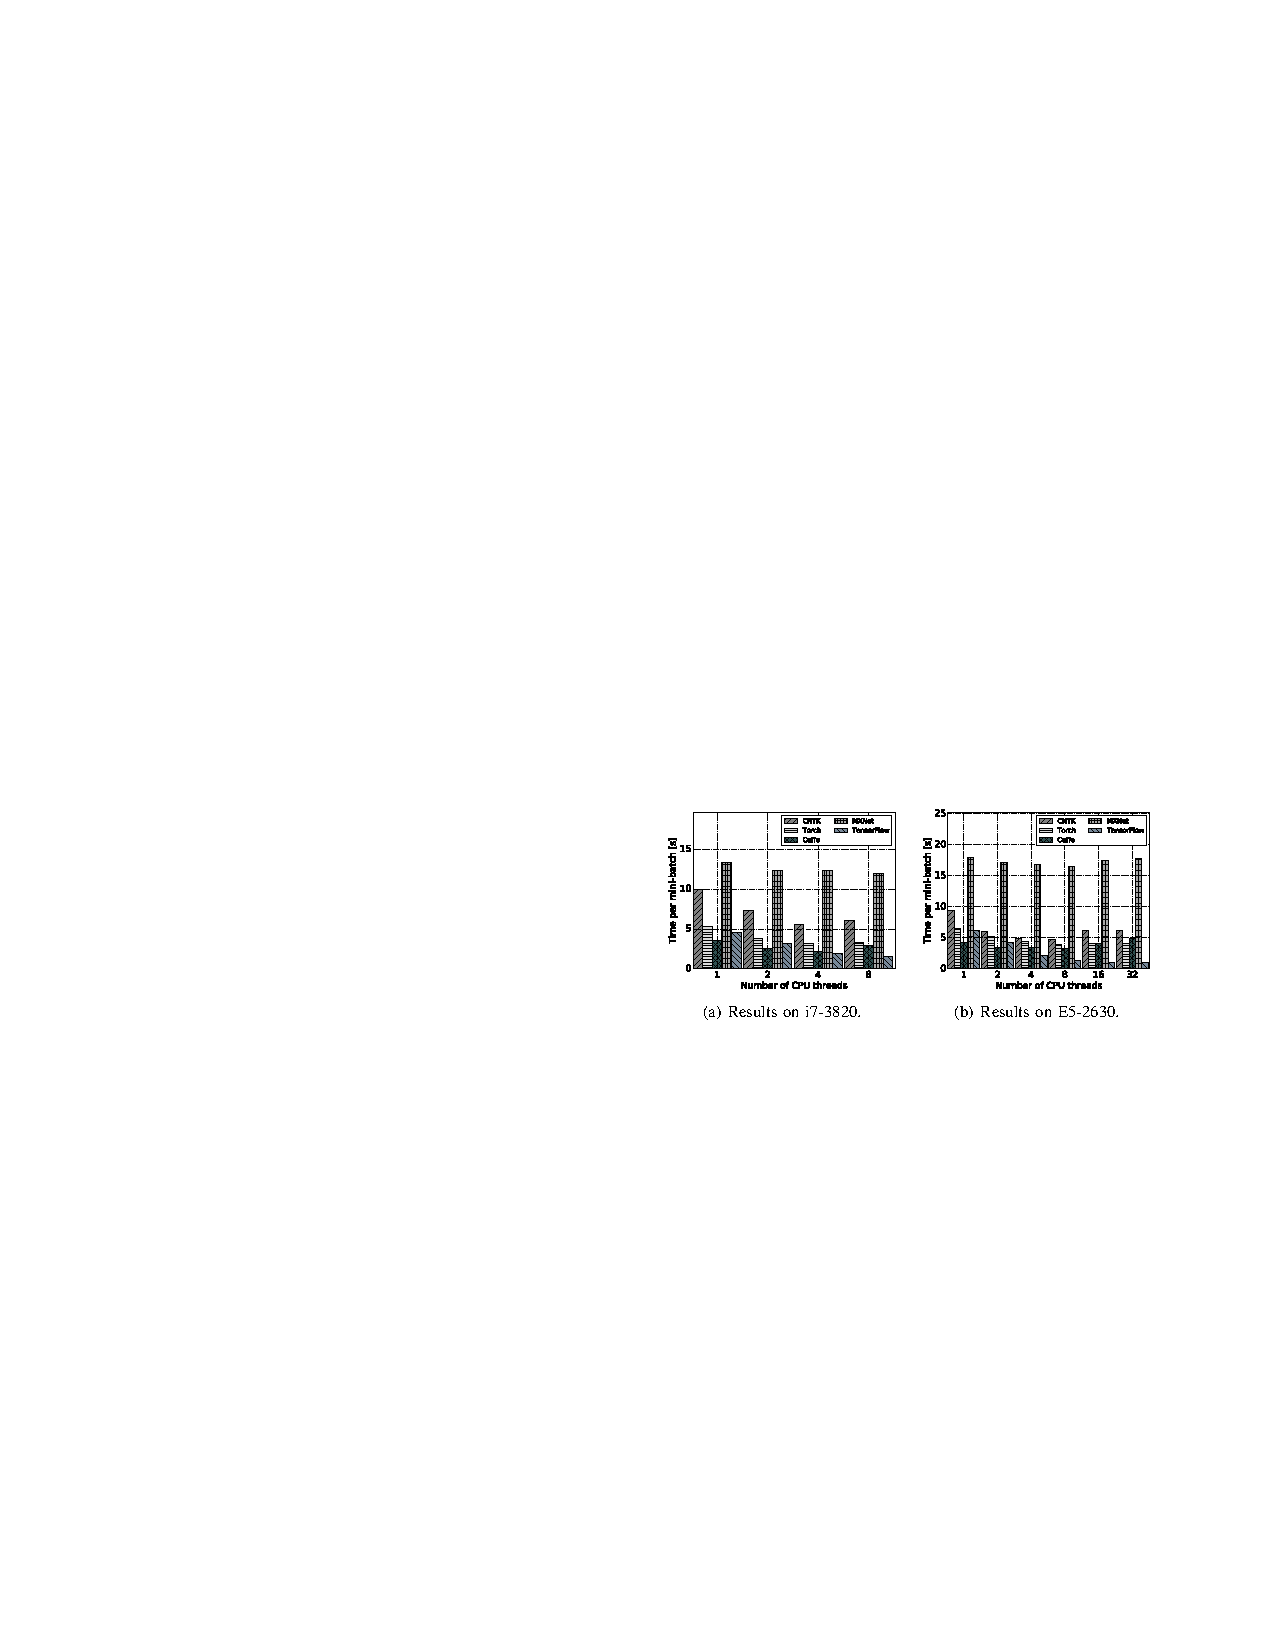
\includegraphics[width=\linewidth]{figures/AlexNet-R1.pdf} 
		\caption{AlexNet-R performance comparison on CPU platform with a mini-batch size of 1024 (The lower the better)}
	\end{figure}
\end{frame}

%%%

\begin{frame}
	\MyLogo
	\frametitle{CPU Scalability: RNN LSTM}  
	\begin{figure}[htbp] 
		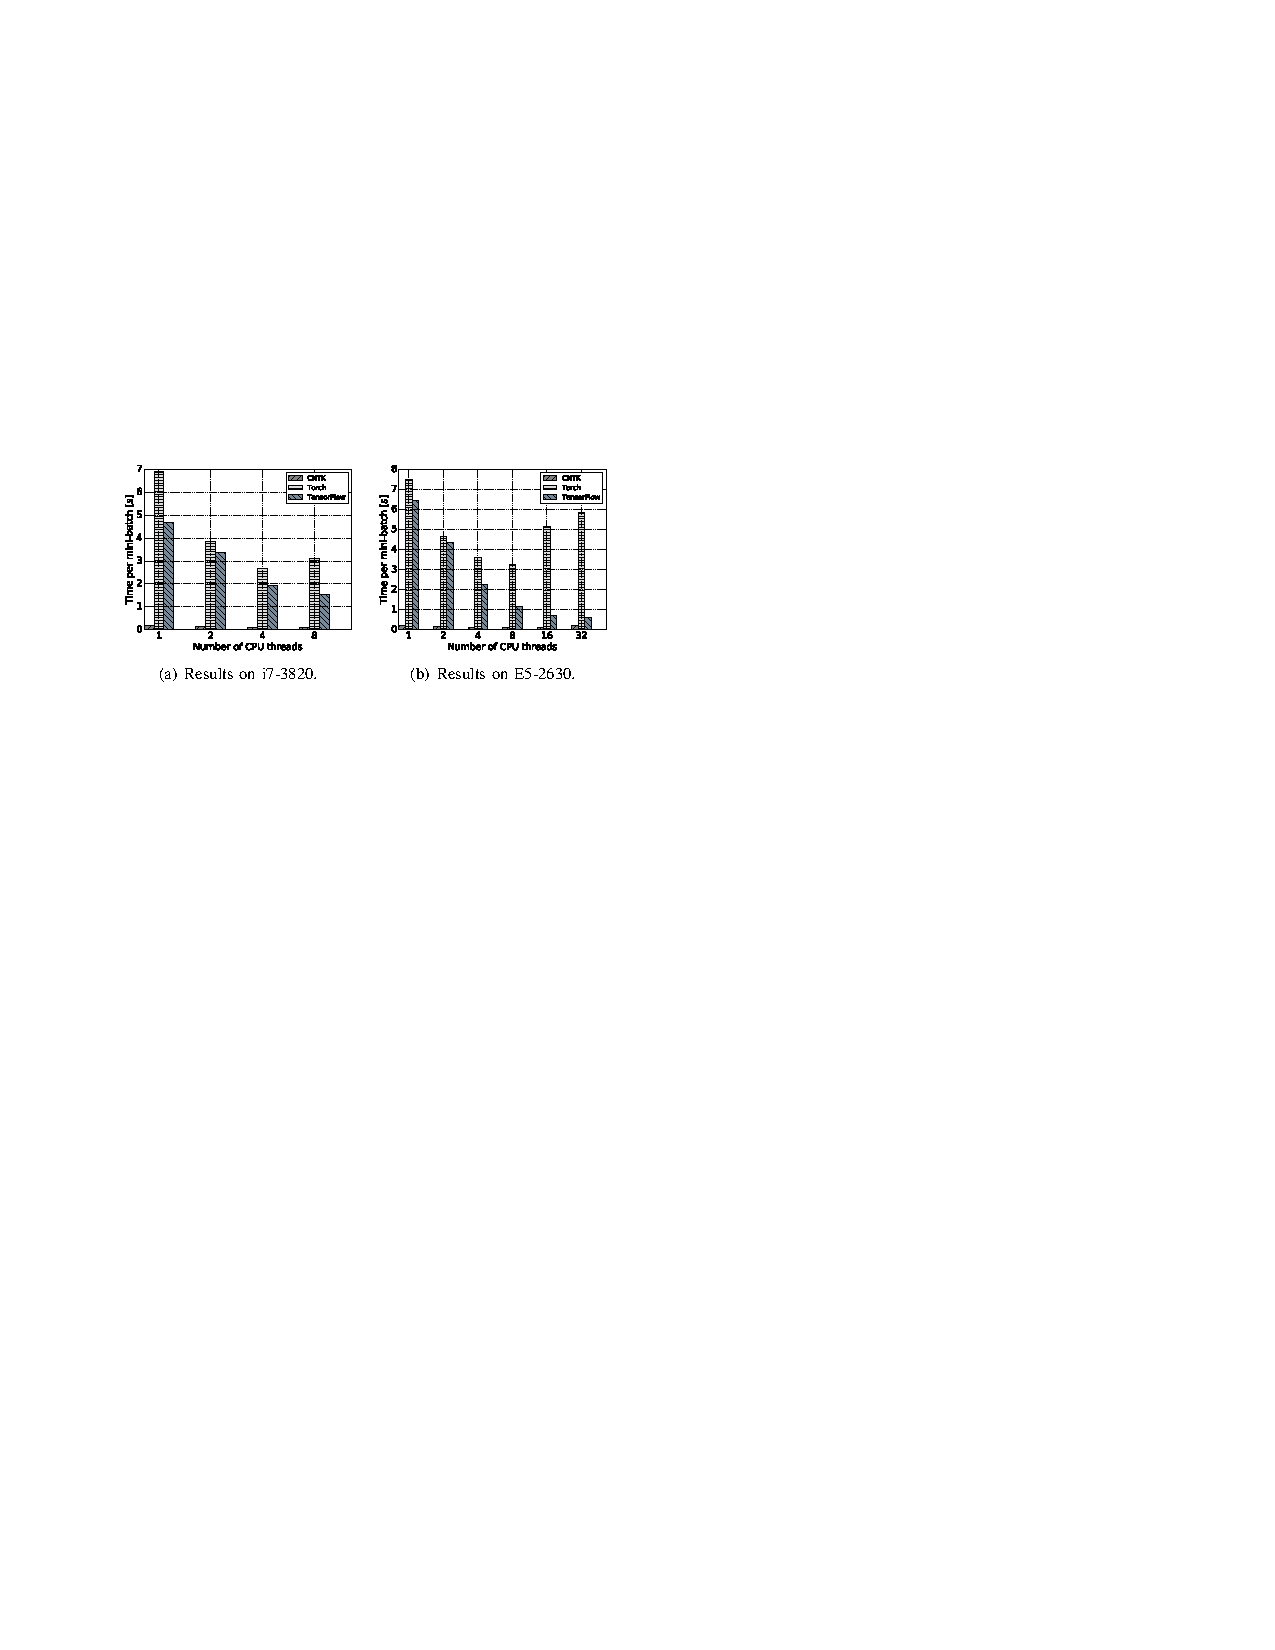
\includegraphics[width=\linewidth]{figures/LSTM1.pdf} 
		\caption{LSTM performance comparison on CPU platform with a mini-batch size of 256 (The lower the better)}
	\end{figure}
\end{frame}

%%%
\subsection{GPU tests}
%%%

\begin{frame}
	\MyLogo
	\frametitle{GPU Scalability: FCN Synthetic}

	\begin{figure}[htbp] 
		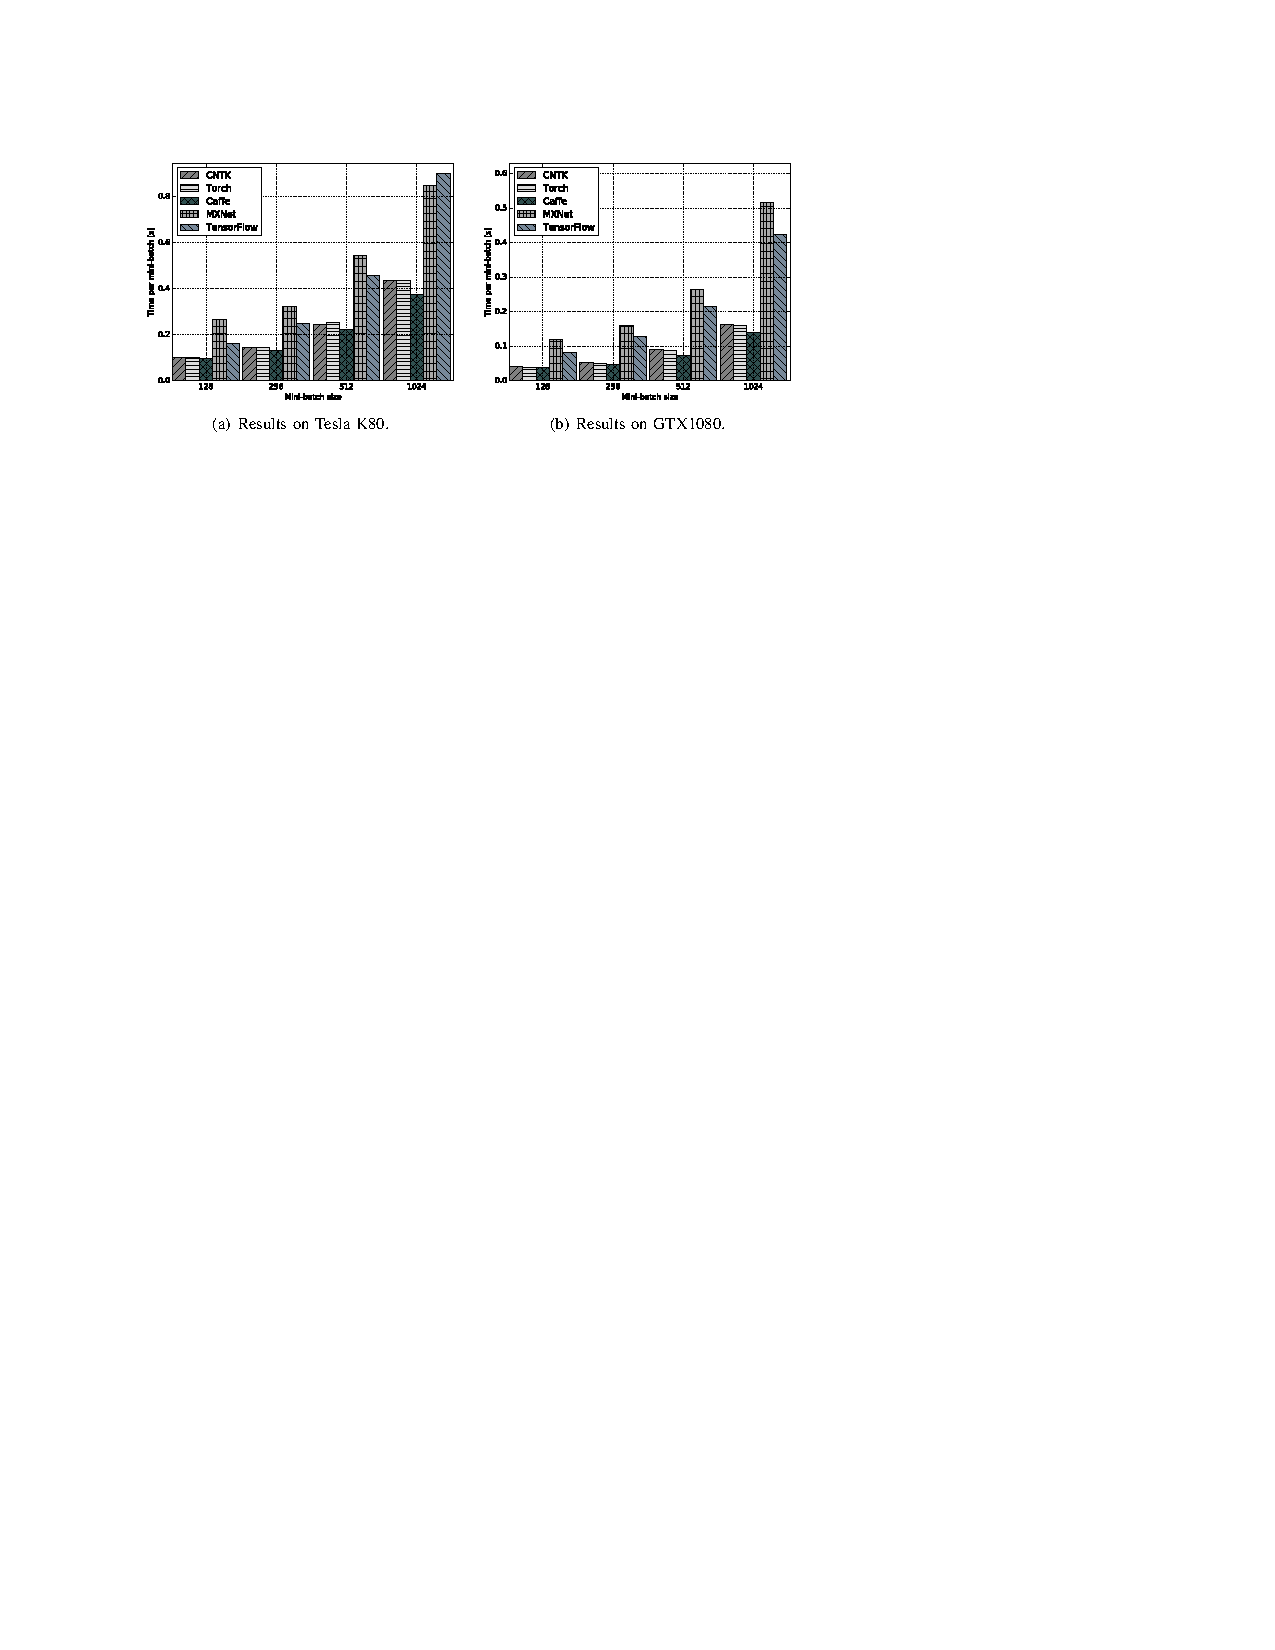
\includegraphics[width=\linewidth]{figures/FCN-S2.pdf} 
		\caption{The performance comparison of FCN-S on GPU platforms}
	\end{figure}

\end{frame}

%%%

\begin{frame}
	\MyLogo
	\frametitle{GPU Scalability: FCN Real}
	
	\begin{figure}[htbp] 
		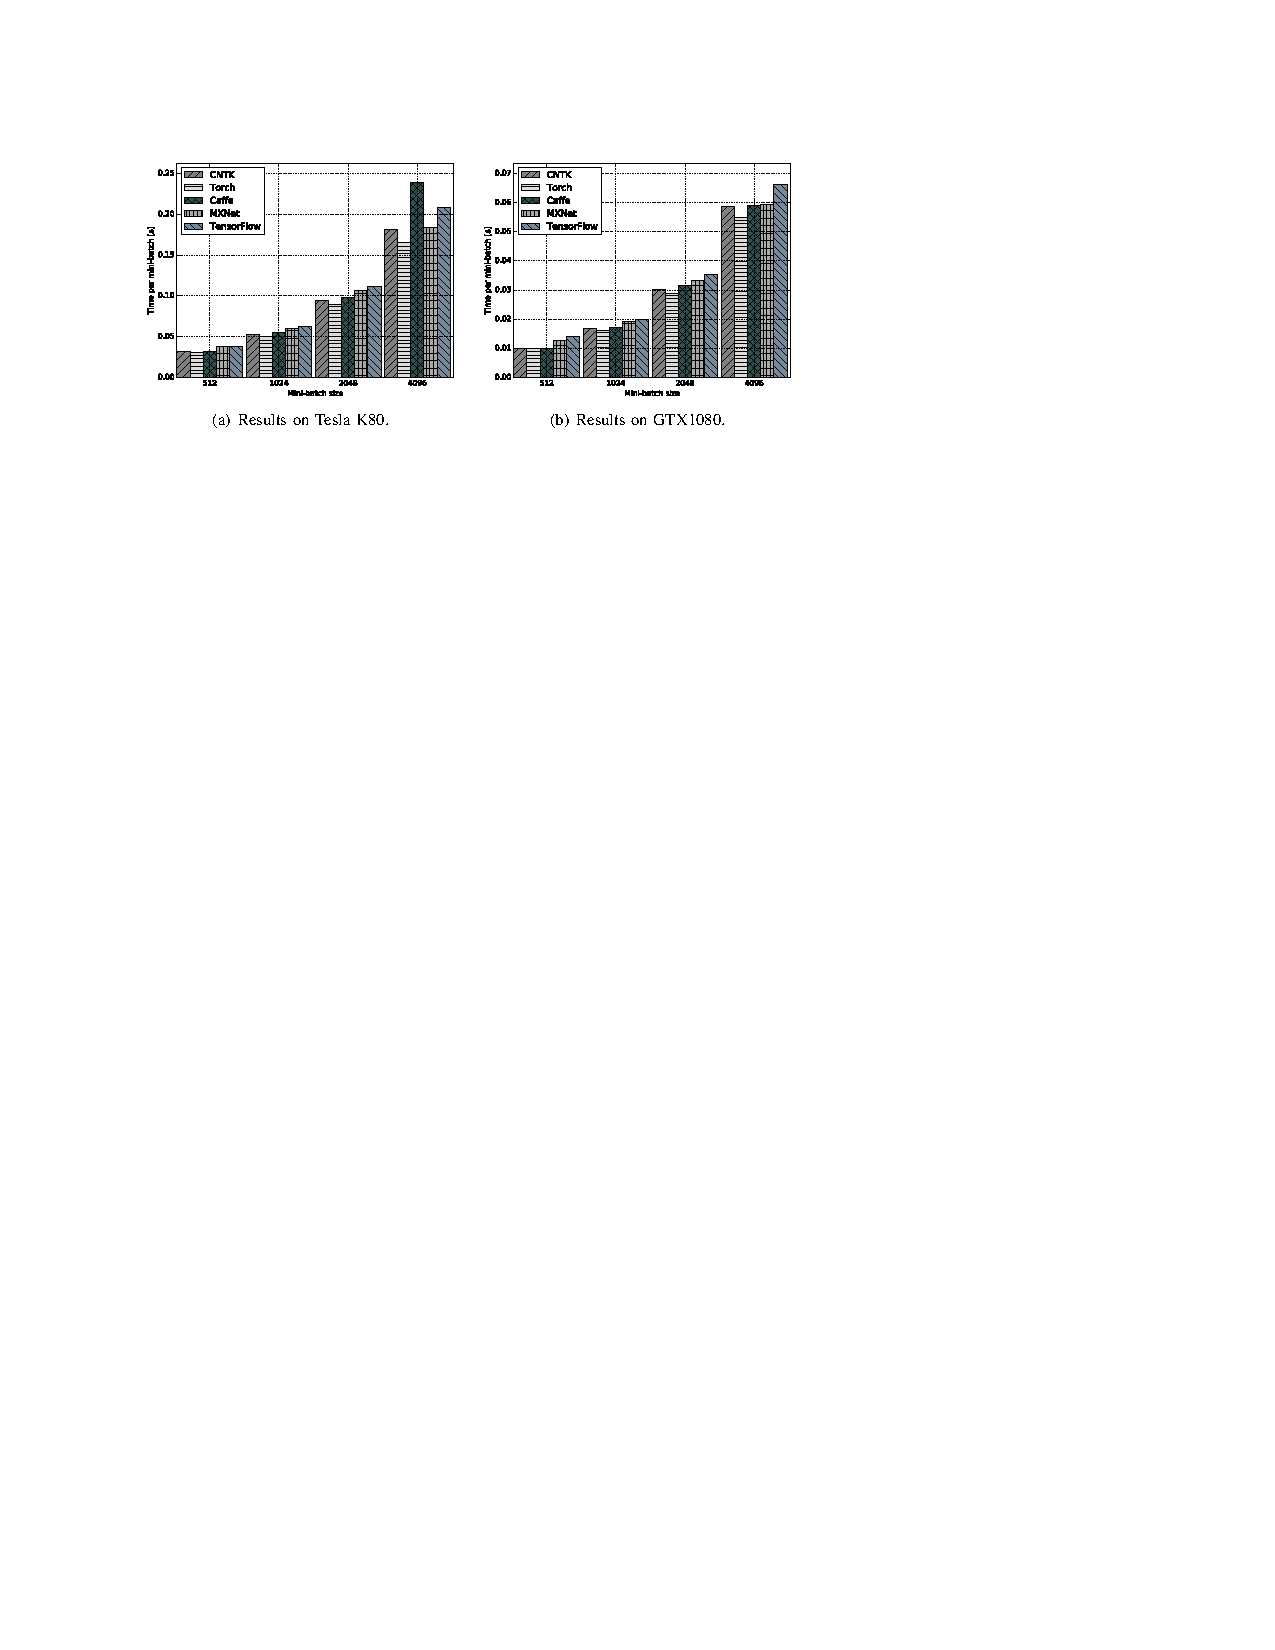
\includegraphics[width=\linewidth]{figures/FCN-R2.pdf} 
		\caption{The performance comparison of FCN-R on GPU platforms}
	\end{figure}

\end{frame}

%%%

\begin{frame}
	\MyLogo
	\frametitle{GPU Scalability: CNN Synthetic}

	\begin{figure}[htbp] 
		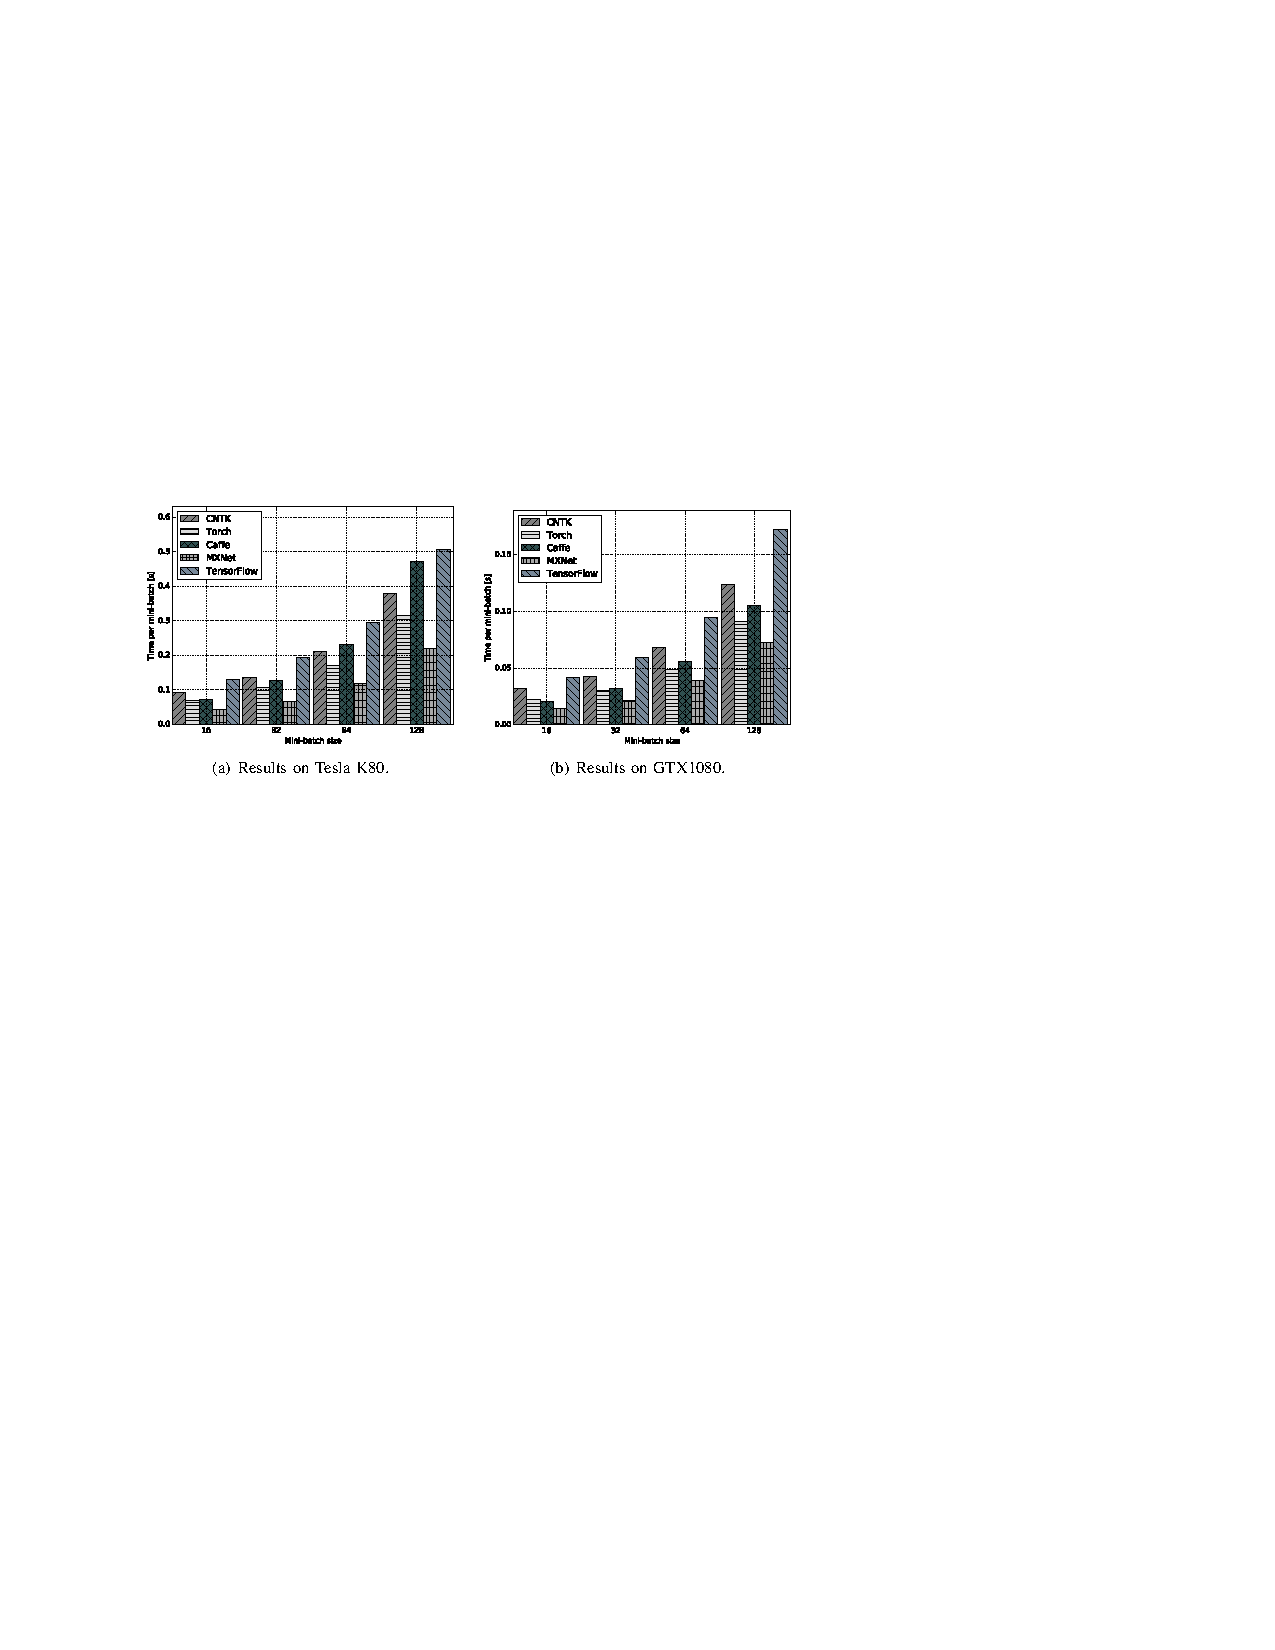
\includegraphics[width=\linewidth]{figures/AlexNet-S2.pdf} 
		\caption{The performance comparison of AlexNet-S on GPU platforms}
	\end{figure}

\end{frame}

%%%

\begin{frame}
	\MyLogo
	\frametitle{GPU Scalability: CNN Real}

	\begin{figure}[htbp] 
		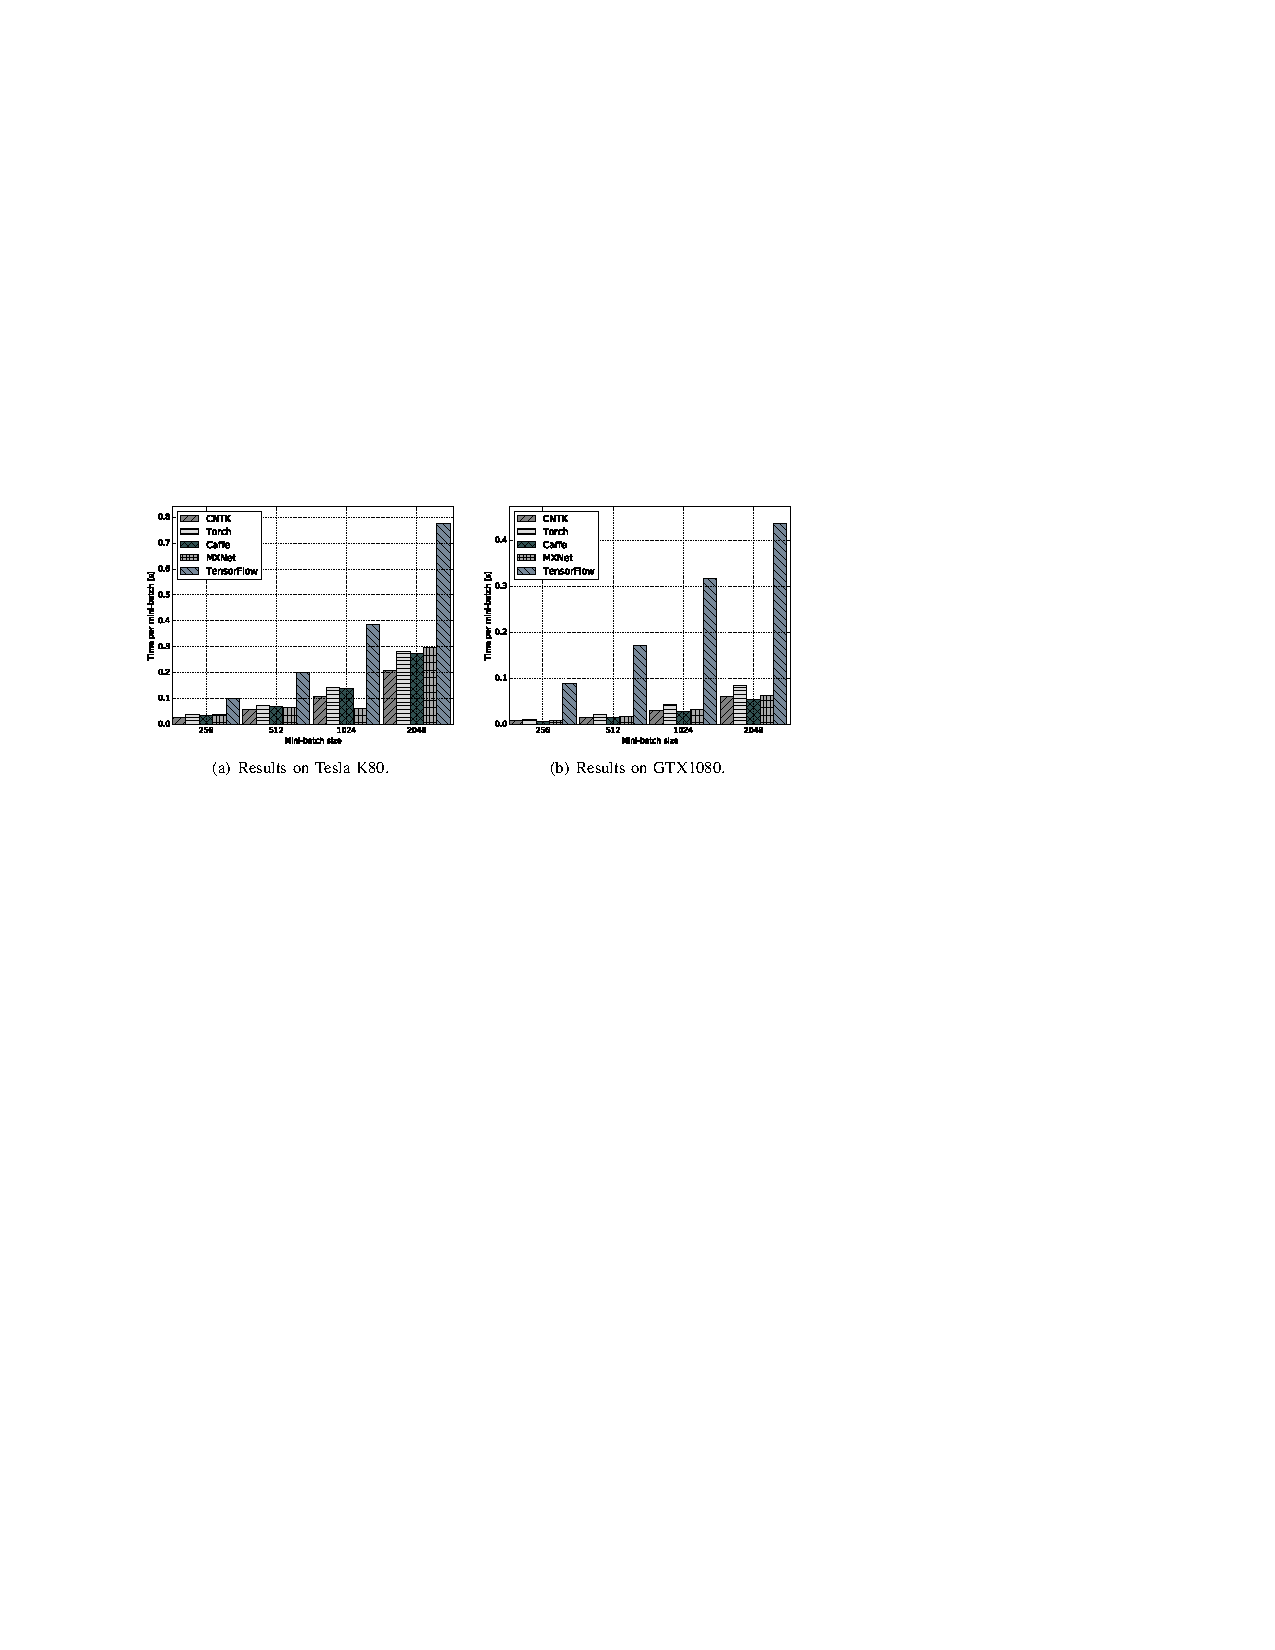
\includegraphics[width=\linewidth]{figures/AlexNet-R2.pdf} 
		\caption{The performance comparison of AlexNet-R on GPU platforms}
	\end{figure}

\end{frame}

%%%

\begin{frame}
	\MyLogo
	\frametitle{GPU Scalability: RNN LSTM}
	
	\begin{figure}[htbp] 
		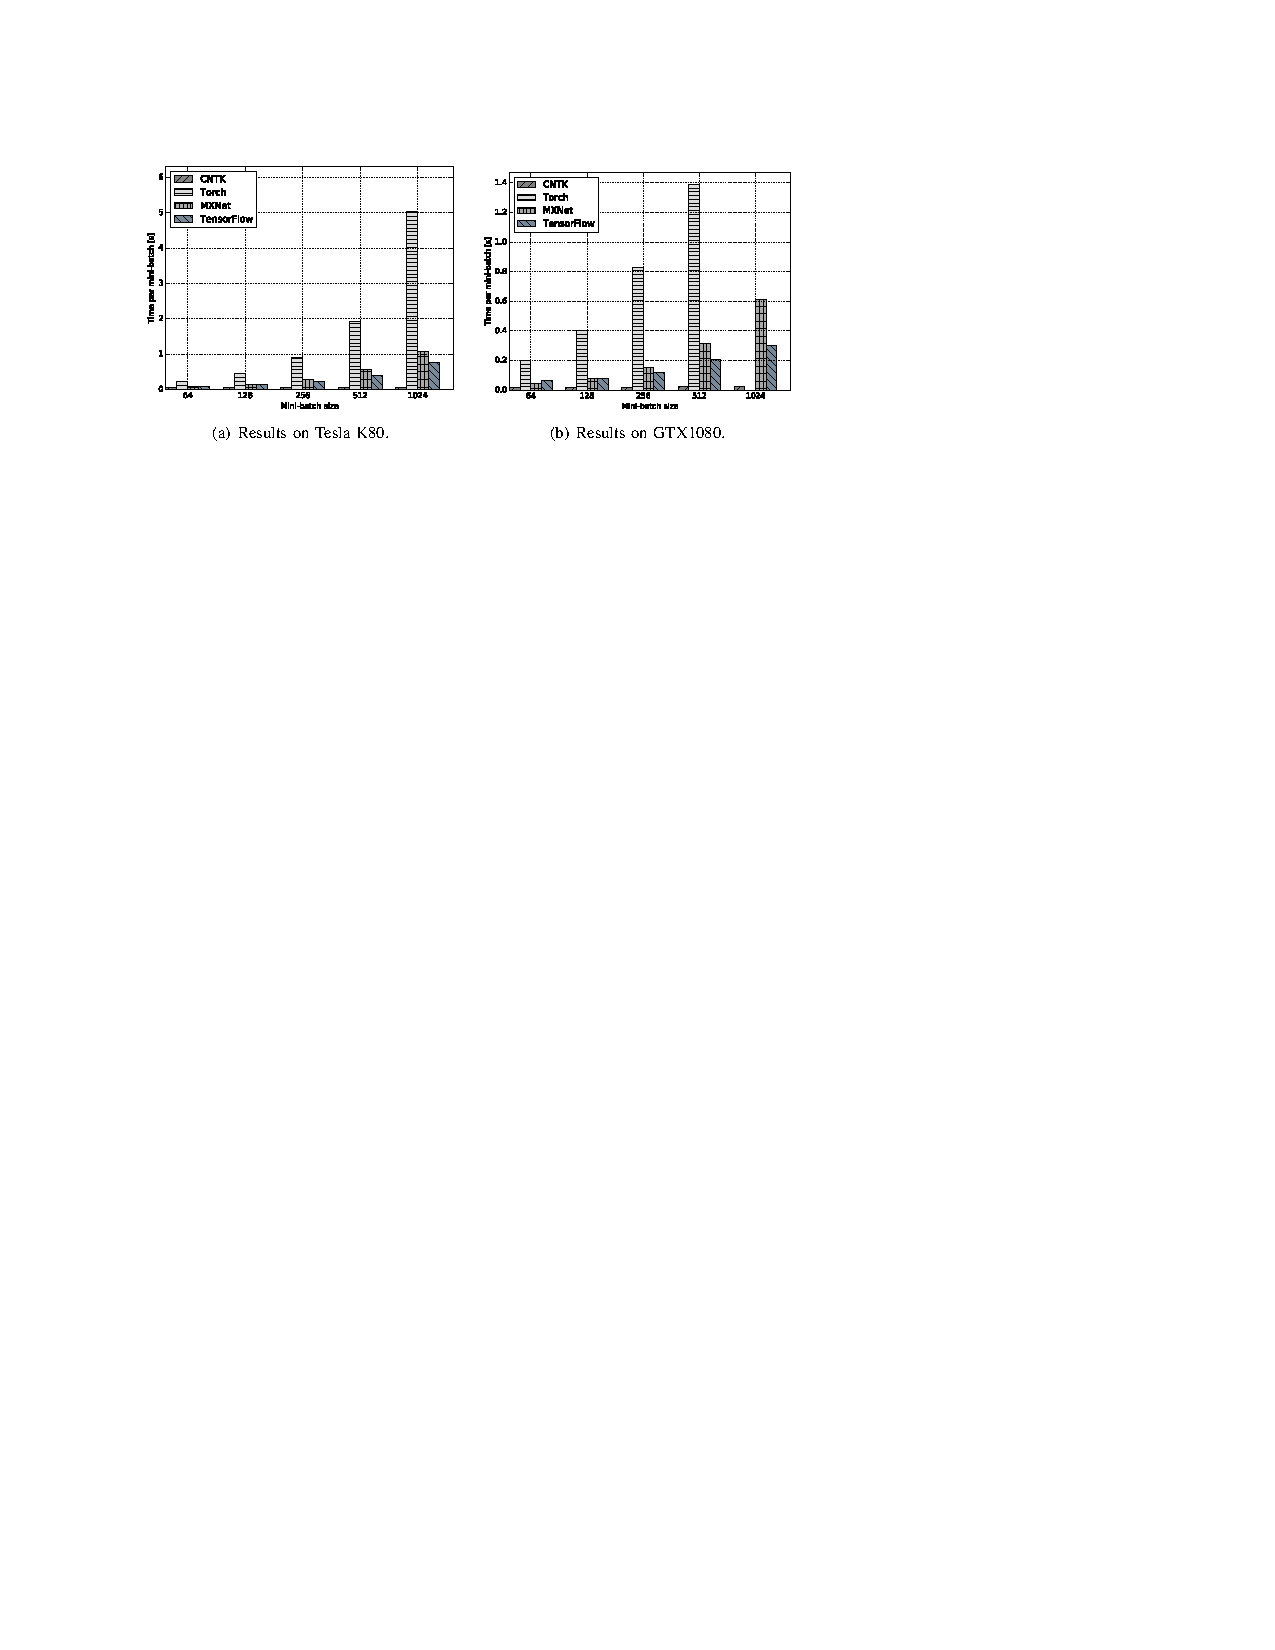
\includegraphics[width=\linewidth]{figures/LSTM2.pdf} 
		\caption{The performance comparison of LSTM on GPU platforms}
	\end{figure}
	
\end{frame}